\documentclass[a4paper]{article}
\usepackage{afterpage}
\usepackage{hanging}
\usepackage{setspace}
\usepackage[a4paper, margin=1.2in]{geometry}
\usepackage{todonotes}
\usepackage{doi}
\usepackage[super,sort&compress,comma]{natbib}
\usepackage{titlesec}
\newcommand{\sectionbreak}{\clearpage}
\bibliographystyle{unsrtnat}
\usepackage{hyperref}
\hypersetup{
    colorlinks=true,
    citecolor=magenta,
    linkcolor=magenta
}
\setlength{\parskip}{0.75em}
\onehalfspacing
\pagestyle{plain}
\graphicspath{ {./figures/} }
\renewcommand{\abstractname}{Summary}

\title{
	{\normalsize Doctoral Thesis Proposal} \\
	{\LARGE \textsc{Building Resilience: How do Species Interactions Shape Ecosystem Collapse?}}
}
\author{
  {\large Fernando Cagua}
}
\date{}

\begin{document}

\maketitle

\begin{abstract}
  Natural ecosystems provide important services---like food and water---we humans depend on to a large extent.
  Much like the failure of a single key financial institution can trigger unexpected crashes on the stock market, human pressures---such as biological invasions and species extinctions---can cause sudden collapses that severely transform the way ecosystems function.
  However, despite its importance, we do not completely understand the dynamics that make ecosystems resilient to collapse.
  Because the functioning of ecosystems is largely determined by the network of interactions between the species that inhabit them, my proposed research aims to quantify the role played by species interactions in determining the resilience of ecosystems.
  To achieve this, I will focus on networks of mutually beneficial interactions, like those between plants and their pollinators, and use a combination of empirical data, computer simulations and ecological theory.
  Ultimately I want to understand why, when and how ecosystem collapses occur, and how to recover from them.
\end{abstract}




\section*{Introduction}
\addcontentsline{toc}{chapter}{Introduction}

From food and freshwater production, to recreation and carbon sequestration, ecosystems provide a wide range of services of considerable value to humans.
Unfortunately, the frequency of undesired ecosystem collapses---like the (often sudden) shift from a transparent to a turbid lake or from a self-sustaining fishery to a collapsed one---is dramatically increasing worldwide\citep{Scheffer2001a}.
When ecosystem resilience is limited, breakdowns are more likely, and their ability to provide those services we depend on is endangered.
Therefore, a necessary step to anticipate, prevent, and reverse ecosystem collapse is to understand the processes that support or undermine ecosystem resilience \citep{Hughes2005, Tylianakis2008}.

Resilience is related to the amount of disturbance that an ecosystem could withstand without collapsing, or, in ecological jargon, undergoing a regime shift---a large, persistent transformation in ecosystem functioning and structure \citep{Holling1973, Gunderson2000}.
Moreover, substantial research indicates that ecosystem functioning and structure are largely determined by the network of interactions formed by species in an ecological community \citep{Bascompte2006, Dobson2006, Tylianakis2008, Reiss2009}.
Since these factors ultimately determine the ecosystem response to disturbances, \textbf{the overall objective of my proposed research is to quantify the role played by species interactions in modulating ecosystem resilience}.

To do so, I will focus on the network of mutualistic interactions between plants and pollinators \citep{Bascompte2006, Bascompte2007, Klein2007}.
These networks, which form the base of pollination systems, play a globally important role in the maintenance of biodiversity and crop production \citep{Bascompte2007, Klein2007}.
Pollination systems are locally important too; for instance two thirds of New Zealand plants are pollinated by birds or insects\citep{Cox2000}, and this includes iconic native plants (like k\={o}whai and p\={o}hutukawa), and economically important crops (like kiwifruit, apples and grapes). However, pollination systems worldwide are currently being disrupted by multiple drivers of human-driven global change \citep{Cox2000}.

Pollination is being affected particularly affected by the simultaneous loss of previously important species, and the introduction of invasive species.
My thesis will concentrate on the resistance and resilience of pollination systems to biotic invasions and defaunation---top components of human-caused global change.
These two drivers have affected New Zealand with particular intensity, at the same time it remains notably vulnerable \citep{Vitousek1997}.
For instance, 50\% of plant species in New Zealand are introduced \citep{Wilton2000}, and imported social bees are now an important component of pollinator fauna \citep{Lloyd1985, Newstrom2005}.
Moreover, the depletion of native birds \citep{Anderson2003, Robertson2009} is a prime example of how pollination systems in New Zealand are losing key pollinators, plants and habitats\citep{Cox2000}.

In the first chapter of my thesis I will concentrate on biotic invasions.
Specifically I have a twofold objective \textbf{first, I aim to determine which network characteristics shape the its resistance and resilience to invasions}, and second \textbf{to determine how biotic invasions, by affecting existing interactions in the community, reshape network resistance and resilience}.
Empirical, time continuous observations of ecosystem dynamics in networks that have been subjected to invasions are limited.
Therefore, I will use computer simulated communities to estimate the population dynamics of the species in the community, and then I will directly quantify stability properties from fluctuations in the species populations \citep{Bastolla2009, Garcia-Algarra2013}.
Specifically I will simulate communities with different network structures, and analyze which structures are more favorable for the coexistence of the invasive species to co-exist in the community.
I will then in turn, see how the structure itself is changed by the invasive species, and whether the change in structure has stability implications.

However, it has been shown that biotic invasions often occur in ecosystems that have already been degraded by species removal \citep{Bennett2015}.
Understanding how invasions interact with defaunation in ecological networks is a global research priority, and essential for conserving, restoring, and managing New Zealand ecosystems \citep{Newstrom2005}.
In the second chapter, I will follow \textbf{by determining the compound effect of biodiversity loss and invasive species on the resilience of an ecosystem}.
I will be extending the models developed in the first chapter, but focusing on how the loss of species---particularly those with a unique role in the ecosystem---make the ecosystem more or less susceptible to invasions.
Simultaneously, the population models will also serve to determine the the patterns of species extinctions that follows after a successful species invasion.

The first two chapters of my thesis are designed to answer underlying questions of resilience theory, however the underlying aim of my third chapter is to translate the gained insight into useful lessons for ecosystem management.
Ecosystems are complex, non-linear systems that are very difficult to control.
However, recent work in theoretical physics has highlighted that is indeed possible to regulate them using targeted interventions \citep{Cornelius2013}.
I propose to build upon these findings to \textbf{determine the optimal set of management actions---from both a theoretical and a feasibility perspective---that are required to modify an ecosystem state}.
For that, using a previously collected empirical dataset that characterized the network of interactions before and after an ecological invasion \citep{Bartomeus2008}, I will first find the set of species that can act as drivers of ecosystem state.
Then, using an extension of the population model developed in the first chapter, I aim to determine the characteristics---like the degree of generalization of trophic position---that make an species more likely to serve as a driver of ecosystem state.
Rescuing ecosystems from the brink of collapse and recovering them from undesired shifts is a major goal in conservation science.
Finding a way in which actions targeted to specific species can maximize the ecosystem resilience, will bring us much closer to that goal.

In a world of constant change, building resilience is our best insurance against losing the ecosystem services we value and depend on.
Although we have identified some of the pervasive effects of invasions and defaunation at the species level, we currently do not understand how the changes on ecosystem dynamics is affecting the resilience of the ecosystems as a whole.
The research I propose intends to establish the general theory necessary to answer this question.
Doing so is especially important when the ecosystem response might be inconspicuous until transformation is imminent.
Only by better understanding the dynamics behind species interactions, can we hopefully be better prepared to anticipate, prevent and reverse undesired ecosystem collapses.




\section{Invasions \& mutualism}
\addcontentsline{toc}{chapter}{Chapter 1}

The invasion of naturalized species is changing ecosystems worldwide.
Fortunately, during the last four decades, there has been steady progress in understanding the causes and outcomes of biotic invasions.
For instance, we now understand that the success of an ecological invasion depends on geographic, bio-climatic, and taxonomic factors, as well as aspects of reproductive biology and general ecology of the introduced organisms.
However, we are still unable to successfully predict the outcome of species introductions in a large proportion of cases.

One of the potential explanations for this limited predictive success is that research on both the causes and consequences of invasive species, have focused on the negative interactions between species in the community (competition, and predator-prey relationships).
However the establishment of an introduced species depends on, or at least is greatly enhanced, by the establishment of  mutualistic relationships \citep{Richardson2000}---in which both interacting species have a positive outcome.
In fact, there are multiple empirical examples of plants that only become successful invaders, when mutualistic partners that pollinate their flowers, or disperse their seeds, are available \citep{Simberloff1999, Simberloff2006, Prior2014}.
Understanding the reciprocal relationship between biotic invasions and mutualism is a key step necessary to both improving current predictions of invasion outcomes, as well as evaluating how invasive species are modifying mutualistic systems \citep{Richardson2000}.

\subsection*{The invasibility of mutualistic systems}

It has been recently shown that there exists a direct link between the structure of ecological networks and ecosystem stability \citep{Bascompte2006,Rooney2006,Okuyama2008,Bastolla2009, Tylianakis2010, Thebault2010,Rohr2014,Sauve2014}.
In particular stable species coexistence in mutualistic networks seems to be favoured by highly diverse, connected, and nested structures \citep{Okuyama2008, Bastolla2009, Thebault2010, Sauve2014}.
For instance, the nested structure observed in many mutualistic networks---in which specialist species tend to interact with a subset of the species with which a generalist interact---support higher amounts of biodiversity, minimise competition among species in the community, and maximise the range of conditions necessary to have a stable community \citep{Bastolla2009, Rohr2014}.
The unambiguous link between ecosystem stability and the ecosystem response to disturbances is an important argument for investigating the implications of network structure and its vulnerability to drivers of global change.

Perturbations caused by global change are severely modifying the structure of mutualistic networks \citep{Burkle2013a}.
Indeed, current evidence suggests that most of its effects are negative \citep{Tylianakis2008, Tylianakis2010}.
Although our understanding of the effects of those perturbations is limited, we know that, for instance, climate change, and habitat modification can lead to shifts on species abundances, and mismatches of phenology, behaviour, or geographic ranges of the interacting species \citep{Memmott2007, Tylianakis2008, Hegland2009, Burkle2013a}.
Those changes can in turn disrupt the patterns of interactions that determine the structure of mutualistic networks.
Some evidence suggest other factors of global change like biotic invasions can also modify the structure of mutualistic networks, for example trough changes in the strength of species interactions, and the degree of network nestedness and connectivity \citep{Olesen2002, Aizen2008, Bartomeus2008, Vila2009, Traveset2013}

I hypothesise that network structure is not only modified by the succesive invasion of alien species, but it also plays an important role in determining the invasibility of the community.
Two facts provide support to this hipothesis.
First, mutualistic interactions are key for the invasion success of introduced species because introduced species need to have suitable pollinators in the new habitat in order to establish themselves in the community \citep{Richardson2000, Sargent2008}.
Second, the structure of mutualistic interactions is known to have direct implications for the number of coexisting species in the community \citep{Moeller2004, Bascompte2006, Bascompte2007, Bastolla2009}.
Specifically, structures that minimise plant competition seem to facilitate species coexistence and promote biodiversity \citep{Bastolla2009}.
Therefore structural attributes---like the degree of specialisation/generalisation, and the contribution to nestedness, of available pollinators---should influence the likelihood an introduced species becomes invasive \citep{Stouffer2014}.

Previous studies have have found that simpler networks, with less species and less interactions between species, are easier to invade \citep{Romanuk2009, Galiana2014}.
However studies are strictly limited to trophic networks in which interactions are chiefly antagonistic (prey-predator) \citep{Romanuk2009, Baiser2010, Galiana2014}.
Lamentably, these results cannot be easily extrapolated because mutualistic interactions introduce facilitation and competition feedbacks that are not present in antagonistic interactions.
Here I will fill that gap, and study the link between different structural attributes of mutualistic networks---degree of nestedness, contribution to nestedness, and compartmentalisation.

The first step to achieve that is to construct simulated communities of mutualistic interactions.
The structure of those communities will be determined by implementing the varying structure of empirically observed networks, as well as by constructing simulated networks with a wide range of structural parameters (\autoref{fig:networks}).
This will allow me to evaluate if the network structures that have been found to minimise competition also make the community more vulnerable to invasions.

\begin{figure}[tbp]
  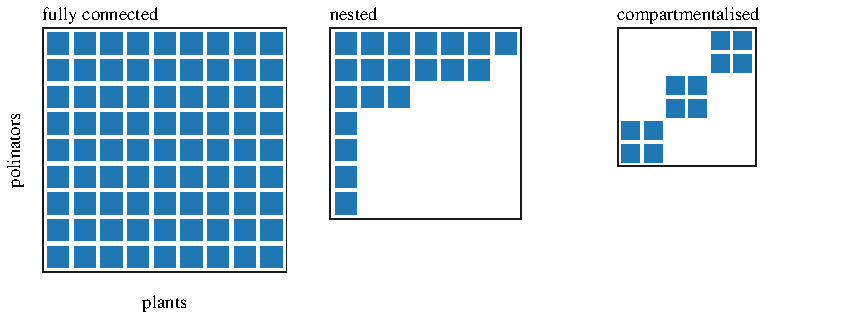
\includegraphics{networks}
  \caption{
  \label{fig:networks}
  Each panel represents a plant–animal network with different network structures.
  Plants compete for resources such as nutrients, but also have indirect interactions mediated by their common pollinators.
  As the number of shared pollinators is higher, positive effects outweigh negative one.
  Current theory predicts a higher number of coexisting species as indicated by the size of the matrices.
  }
\end{figure}

The second step is to develop models of the population dynamics in mutualistic communities in which the abundances of each species present on the community depends on their growth rate ($births - deaths$).
These growth rates can in turn be affected by the feedbacks imposed by the interactions with other species.
Previous theoretical work has largely assumed that the feedbacks of mutualistic interactions increase the growth rates of the focal species, while antagonistic interactions decrease it, which in turns allows the coexistence of a larger number of species (\autoref{fig:networks}) \citep{Moeller2004, Bastolla2009}.

This assumption, however, ignores that in mutualistic systems, organisms might also compete to optimise the obtained benefits.
Indeed evidence suggest that in plant-pollinator systems, the increase of mutualistic interactions caused by invasive species, does not translate in increased facilitation \citep{Lopezaraiza-Mikel2007}.
Because plant reproduction depends strongly in the quality of the mutualistic service, mutualisms can be strongly altered when co-flowering species compete for the service of shared pollinators \citep{Sargent2008, Mitchell2009}.
This happens because the visit of a pollinator does not lead to reproduction if pollen is transfered between different species of plants \citep{Morales2008}.
Even though there are some mechanisms to mitigate the impacts of competition for mutualism and inter-specific pollen transfer \citep{Ghazoul2006, Bartomeus2008a}, it has been found that invasive species, at high densities, are able to co-opt pollinators from native species \citep{Pysek2011}, dominate the networks of pollen transport \citep{Lopezaraiza-Mikel2007, Alarcon2010}, and ultimately decrease the seed output of native species \citep{Munoz2008}.

The third step is to analyse the ecosystem response to an alien species.
Depending on the network structure, and the traits of the native and alien species, the outcome of an species introduction can vary.
One possible outcome option is that alien species is not able to invade the community(\hyperref[fig:dynamics]{Figure \ref{fig:dynamics}a}).
Another possibility is that the alien species becomes an invader, which can, in some instances, have catastrophic consequences for other species in the community (\hyperref[fig:dynamics]{Figure \ref{fig:dynamics}b, c}).
respond.
Therefore, I will quantify the invasibility of the community as the likelihood that an invader is successful \citep{Ives2007, Romanuk2009}.

\begin{figure}[tbp]
  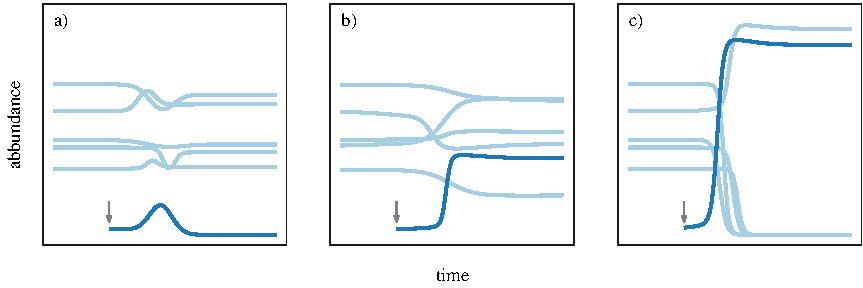
\includegraphics{dynamics}
  \caption{
  \label{fig:dynamics}
  Three possible responses of ecosystems in stable coexistence to the introduction of an alien species (dark blue):
  a) the alien species did not succeed to coexist, and caused only minor changes in the abundances of the species already present in the community (light blue);
  b) the alien species persisted with the original species; or
  c) the alien species became invasive, and five of the original species went extinct.
  }
\end{figure}

Because, as mentioned, a nested structure maximises the number of species that can stably coexist \citep{Bastolla2009}, I predict that a similar relationship exists between invasibility and nestedness.
However, I also argue that the competition for pollinators confers the community a resistance to invasions that has not been accounted for in previous theoretical or empirical research (\autoref{fig:hypo_c1}).
These hypotheses link concepts of network structure, apparent competition/facilitation and ecosystem stability, and will allow us to put limited and somewhat disparate empirical observations in context.

Despite the general belief that successful invasive species tend to be super-generalists \citep{Richardson2000, Aizen2008, Vila2009, Albrecht2014}, a recent meta-analysis has shown that invasive species become very integrated in pollination networks \citep{Stouffer2014}.
Specifically, invasive plants seem to interact preferentially with pollinators that are weak contributors to community nestedness, which have been shown to be the less vulnerable to extinction \citep{Saavedra2011, Stouffer2014}.
However this empirical observation has not yet been explained mechanistically.
By testing the hypotheses I propose, not only light will be shed on what makes ecosystem vulnerable to invasions, but also, because they deal with fundamental tenets in theoretical ecology, we will also gain a better understanding of the implications of network structure on the persistence of biodiversity, the link between stability and biodiversity, and the assembly of ecological communities.

\begin{figure}[tbp]
  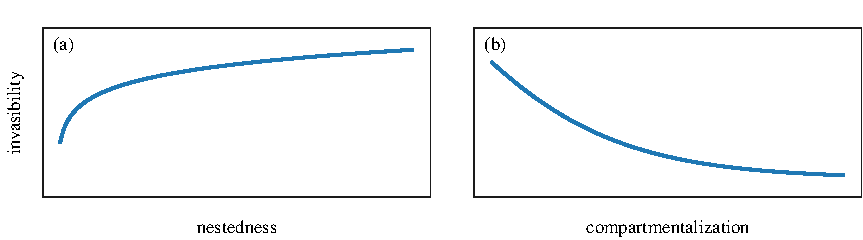
\includegraphics{hypo_c1}
  \caption{
  \label{fig:hypo_c1}
  It has been found that a) an increasingly nested structure enhances the number of species that can stable coexist, while b) a compartmentalized structure decreases it.
  I hypothesise that a similar relationship exist between these attributes of network structure and the invasibility of the community.
  In addition, I argue that the apparent competition for pollinators increases the resistance of mutualistic communities to invasions by counteracting the positive feedbacks of apparent facilitation.}
\end{figure}

\subsection*{Invasions change the structure of mutualistic networks}

After analyising the structures that make an ecological network more or less susceptible to invasions, I then follow by investigating the consequences for the community when the invasion is successful (\autoref{fig:diagram_c1}). On one hand, I will explore the feedbacks on the structure of mutualistic network after an successful invasion; on the other hand I will explore when the invasions lead to a large number of secondary extinctions and ultimately ecosystem collapse (\hyperref[fig:dynamics]{Figure \ref{fig:dynamics}c}).

\begin{figure}[tbp]
  \centering
  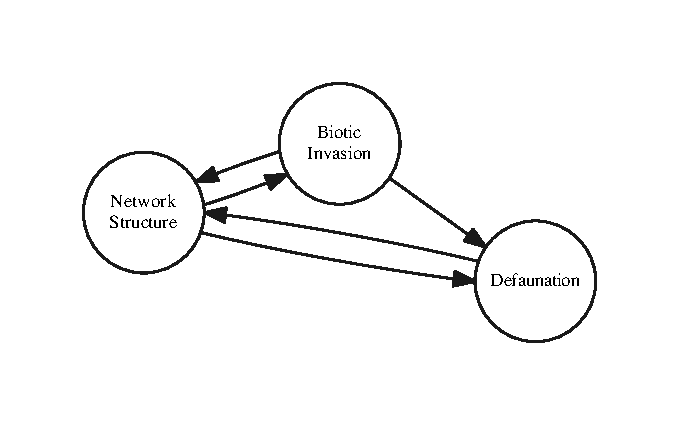
\includegraphics{diagram_c1}
  \caption{
  \label{fig:diagram_c1}
  The network structure determines the invasibility of an ecological community.
  However, successful invasions also modify the structure itself, whether trough a shift in interaction partners or trough secondary extinctions in the community.
  }
\end{figure}

Successful invasive species have been shown to have pollination effects in the native species trough changes on pollinator populations and behavior \citep{Christian2001, Bjerknes2007, Morales2009, Vila2009}.
Although, as mentioned, they can have facilitative effects by increasing the total visitation rates \citep{Bjerknes2007, Sargent2008}, they can also have negative effects by decreasing con-specific or increasing hetero-specific pollen transfer \citep{Morales2009}.
Therefore, changes on the structure of networks are expected.

Although there are few empirical studies that measure the consequences of ecological invasions in network structure, evidence suggest that invasive species have indeed the ability to modify the structure of mutualistic networks.
In particular, invaded communities seem to be more nested \citep{Bartomeus2008, Stouffer2014} and less compartmentalised \citep{Albrecht2014} than their un-invaded counterparts , while also having altered visitation patterns \citep{Vila2009}.
However results are somewhat contradictory \citep{Gilberto2012}, and the limited amount of evidence precludes the generalisation of the patterns observed.

I will use the theoretical results obtained from the population dynamics model to fill the gap on empirical data.
Specifically I will quantify the changes on network structure (nestedness, and compartmentalisation) induced by the invasive species, and the contribution to structure of both the invasive species, and the species it interacts with \citep{Saavedra2011, Stouffer2014}.
Therefore, it will be possible to quantify how an initial successful invasion affects the future invasibility of the community.
However a successful invasion can, not only affect future invasibility by causing changes on network structure, but also by causing extinction cascades that disrupt mutualisms in the community \citep{Christian2001, RodriguezCabal2013}.

It is also possible to quantify the stability of an ecosystem by measuring the number of species extinctions that follow a successful invasion \citep{Post1983, Ives2007}.
Paradoxically, the same structures that I propose are the most vulnerable to invasions, have also been shown to be the most robust to cascading extinctions in ecological networks \citep{Tylianakis2010, Stouffer2011, Albrecht2014}.
The research I propose will help disentangle these two seemingly disparate observations.

\section{Combined effects of global change}
\addcontentsline{toc}{chapter}{Chapter 2}

Random or top down, down-top, not functional

\end{figure}
\section{Controlling ecological networks}
\addcontentsline{toc}{chapter}{Chapter 3}

sdfxc

\section*{Research Plan}
\addcontentsline{toc}{chapter}{Research Plan}

asd

\footnotesize
\twocolumn
\bibliography{../../references}
\addcontentsline{toc}{chapter}{References}

\end{document}
